% ===== c08 第 18 节「半正交分解」 p029–p032 =====
% 页面图像上实际编号公式 42 条：(17.11)(17.12) + (18.1)–(18.40)。
% p029 上半页为第 17 节末尾的箭图 (17.11)(17.12) 与图 17.1–17.3；第 18 节标题自 p029 中部起。

\begin{equation}
  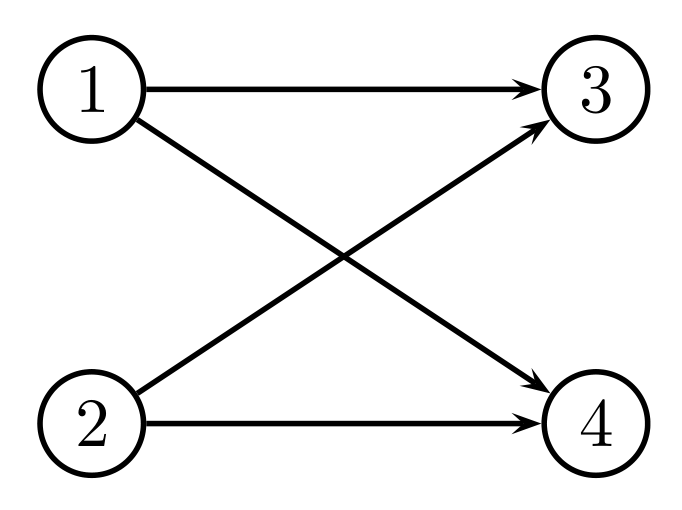
\includegraphics[width=0.24\textwidth]{figures/eq17.11.png}
  \tag{17.11}
\end{equation}

\begin{equation}
  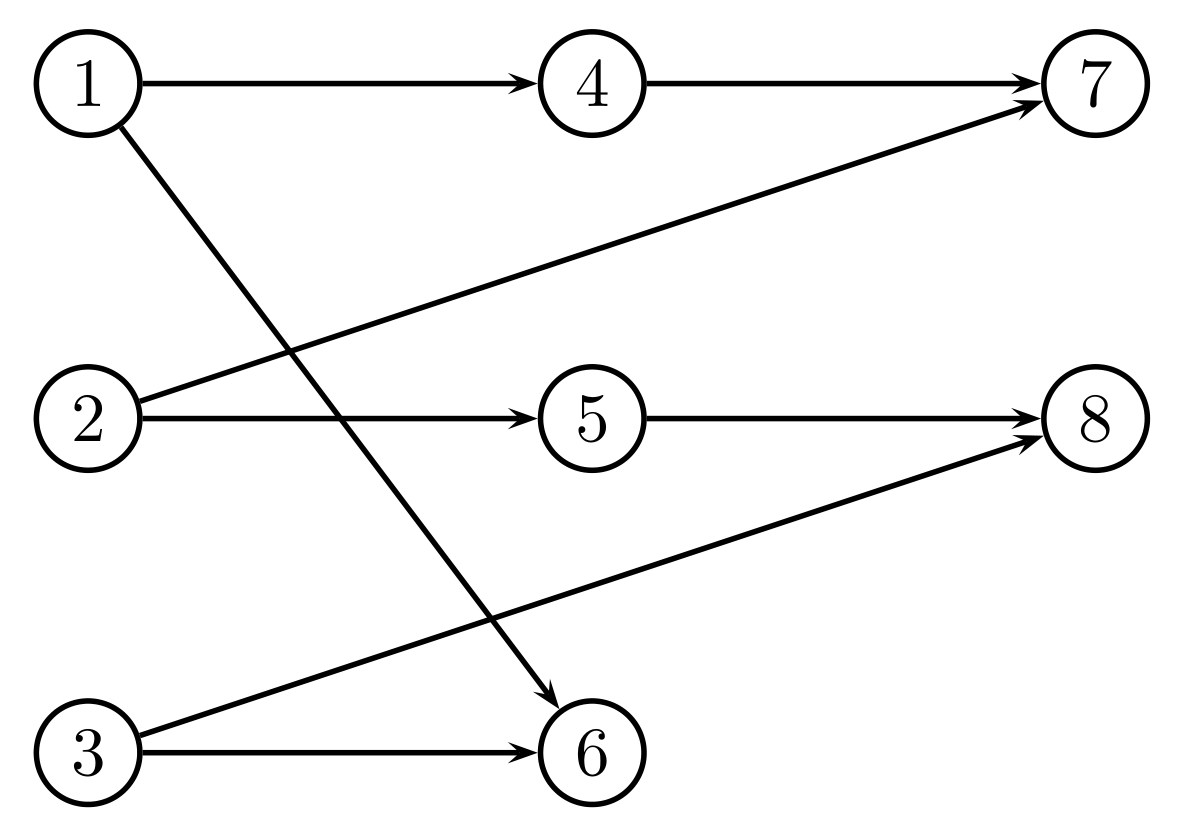
\includegraphics[width=0.41\textwidth]{figures/eq17.12.png}
  \tag{17.12}
\end{equation}

% [Tutor Note: (17.11)(17.12) 为箭图（quiver）示意，原书以图元绘制；preamble 未加载 tikz，故按页面裁图原样嵌入（work/figures/eq17.11.png、work/figures/eq17.12.png），节点编号与箭头方向均未改动。]

\begin{figure}[htbp]\centering
  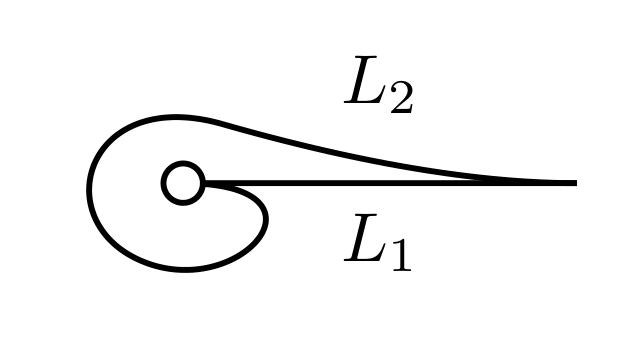
\includegraphics[width=0.28\textwidth]{figures/fig17.1.png}
  \figtitle{17.1}{$(a,b)=(1,1)$}
\end{figure}

\begin{figure}[htbp]\centering
  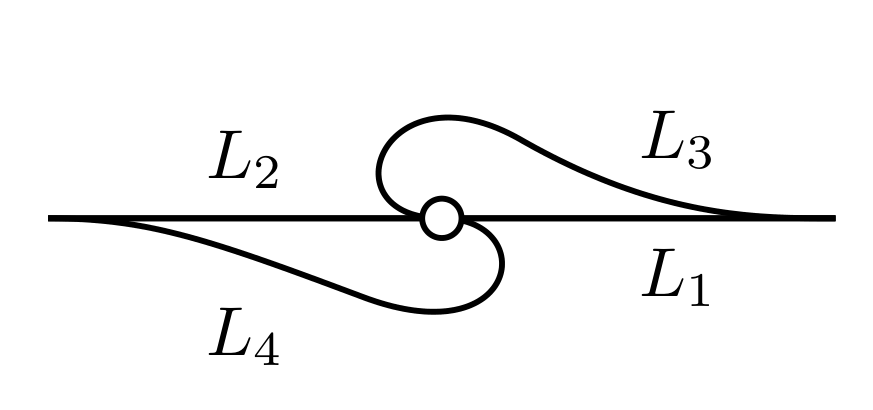
\includegraphics[width=0.34\textwidth]{figures/fig17.2.png}
  \figtitle{17.2}{$(a,b)=(1,1)$}
\end{figure}

\begin{figure}[htbp]\centering
  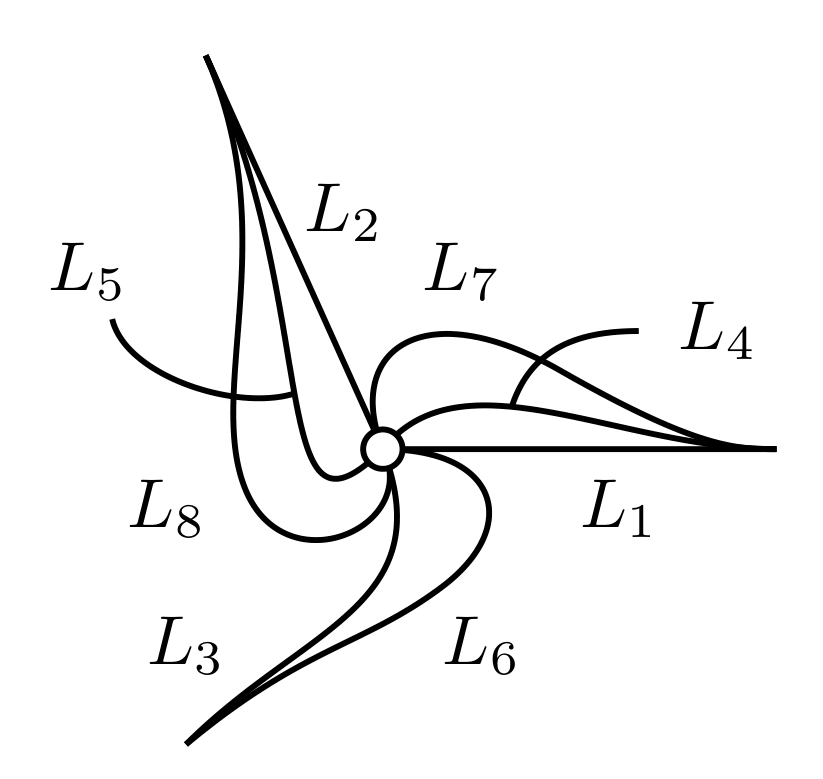
\includegraphics[width=0.31\textwidth]{figures/fig17.3.png}
  \figtitle{17.3}{$(a,b)=(1,1)$}
\end{figure}

% [Tutor Note: 原文図 17.2、17.3 的图注亦印作 (a,b)=(1,1)，而 p028 正文称三图分别对应 (a,b)=(1,1),(2,2),(3,5)；图注疑为原文误植，此处照图注原样保留。]

\section{半正交分解}

三角范畴 $\cT$ 的全子范畴 $\cN$ 称为右可容许的（right admissible），是指嵌入函子 $i\colon\cN\hookrightarrow\cT$ 具有右伴随函子 $i^{!}\colon\cT\to\cN$。同样地，当嵌入函子具有左伴随函子 $i^{*}\colon\cT\to\cN$ 时，称为左可容许的（left admissible）。$\cN$ 为右可容许的充要条件是：对任意 $X\in\cT$，存在正合三角 $N\to X\to M$，使得 $N\in\cN$ 且 $M\in\cN^{\perp}$。当 $\cT$ 与 $\cN$ 具有 Serre 函子时，

\begin{align}
  \Hom_{\cT}(X,i(N)) &\cong \Hom_{\cT}(i(N),S_{\cT}(X))^{\vee} \tag{18.1}\\
  &\cong \Hom_{\cN}(N,i^{!}\circ S_{\cT}(X))^{\vee} \tag{18.2}\\
  &\cong \Hom_{\cN}(i^{!}\circ S_{\cT}(X),S_{\cN}(N)) \tag{18.3}\\
  &\cong \Hom_{\cN}(S_{\cN}^{-1}\circ i^{!}\circ S_{\cT}(X),N) \tag{18.4}
\end{align}

由此

\begin{equation}
  i^{*} \cong S_{\cN}^{-1}\circ i^{!}\circ S_{\cT} \tag{18.5}
\end{equation}

从而左右可容许性等价。双侧可容许子范畴简称为可容许子范畴（admissible subcategory）。当存在可容许子范畴的序列 $(\cN_1,\dots,\cN_n)$ 与左可容许子范畴的递增序列 $\cT_1=\cN_1\subset\cT_2\subset\dots\subset\cT_n=\cT$，且对任意 $i=1,\dots,n-1$，$\cN_i$ 在 $\cT_i$ 中与 $\cT_{i-1}$ 左正交时，

\begin{equation}
  \cT = \langle \cN_1,\dots,\cN_n \rangle \tag{18.6}
\end{equation}

并称 $\cT=\langle\cN_1,\dots,\cN_n\rangle$ 为 $\cT$ 的半正交分解（semiorthogonal decomposition）。

三角范畴的对象 $E$ 若满足

\begin{equation}
  \Hom^{i}(E,E) =
  \begin{cases}
    \C\cdot\id_{E} & i=0,\\
    0 & \text{otherwise}
  \end{cases} \tag{18.7}
\end{equation}

则称为例外对象（exceptional object）。若例外对象的序列 $(E_1,\dots,E_n)$ 对任意 $i>j$ 与 $k\in\Z$ 满足

\begin{equation}
  \Hom^{k}(E_i,E_j) = 0 \tag{18.8}
\end{equation}

则称为例外序列（exceptional sequence）。由例外序列作为三角范畴生成的子范畴必定是可容许的。当例外序列生成 $\cT$（作为三角范畴）时，称为完备的（full）。对完备例外序列 $(E_1,\dots,E_n)$，设 $E_i$ 生成的 $\cT$ 的三角子范畴为 $\cN_i$，则存在 $\cT$ 的半正交分解 $\cT=\langle\cN_1,\dots,\cN_n\rangle$，并记作 $\cT=\langle E_1,\dots,E_n\rangle$。此时 $\cT_i$ 是由 $E_1,\dots,E_i$ 生成的 $\cT$ 的三角子范畴。

给定微分分次范畴 $\cD$ 及其上对象的序列 $(E_1,\dots,E_n)$ 时，以这些对象为对象的新微分分次范畴 $\cD^{\to}$ 定义为

\begin{equation}
  \hom_{\cD^{\to}}(E_i,E_j) :=
  \begin{cases}
    \C\cdot\id_{E_i} & i=j,\\
    \hom_{\cD}(E_i,E_j) & i<j,\\
    0 & \text{otherwise}
  \end{cases} \tag{18.9}
\end{equation}

并称之为关于 $(E_1,\dots,E_n)$ 的 $\cD$ 的有向子范畴（directed subcategory）。有向子范畴是非全子范畴的重要例子。此外，当 $\cD$ 是 Calabi–Yau 范畴（即在 $\mathrm{Ho}\,\cD$ 中 Serre 函子为整数平移的范畴），且 $(E_1,\dots,E_n)$ 通过映射锥与直和因子生成 $\cD$ 时，存在与取有向子范畴相逆的操作，称为 Calabi–Yau 扩张（Calabi–Yau extension）。这是从类似于 Fano 流形的相干层的导出范畴的范畴出发，构造类似于 Calabi–Yau 流形的相干层的导出范畴的范畴的操作。Calabi–Yau 扩张有平凡的情形 [Seg08, Bal] 与非平凡的情形 [Kel11]。例如，当 $\cD^{\to}$ 是 $\PP^{2}$ 的相干层的导出范畴、且 $(E_1,E_2,E_3)=(\cP_{\PP^{2}},\cP_{\PP^{2}}(1),\cP_{\PP^{2}}(2))$ 时，作为 $\cD^{\to}$ 的 1 维非平凡 Calabi–Yau 扩张可得椭圆曲线的相干层的导出范畴，作为 3 维平凡的 Calabi–Yau 扩张可得 $\PP^{2}$ 的典范丛的全空间的相干层的导出范畴。

% [Tutor Note: 原文此处作花体 𝒫_{P²}（即 \cP_{\PP^{2}}），按 Beilinson 例外列通常应为 𝒪_{P²}；此处照录原文，请审校确认。]

有向子范畴的导出范畴按定义具有完备例外序列，Fukaya–Seidel 范畴正是其例。由同调镜像对称，这与 [Kaw06b] 关于完备环面流形的相干层的导出范畴具有完备例外序列的结果相对应。此外，去掉若干例外对象即可得到可容许子范畴，人们期待这与极小模型理论中的收缩、flop 相对应 [Kaw13, BFK, BO, BO02, Kuzb]。[AKO08] 利用这一点证明了 Hirzebruch 曲面的同调镜像猜想。另外，[Ker08] 考察了对应于环面曲面的加权爆破的镜像的行为。

对于半正交分解

\begin{equation}
  \cT = \langle \cN_1,\cN_2 \rangle \tag{18.10}
\end{equation}

称 $\phi = i_2^{*}\circ i_1\colon\cN_1\to\cN_2$ 为粘贴函子（gluing functor）。例如，设 $\PP^{2}$ 的单点爆破为 $\pi\colon X\to\PP^{2}$，则 $X$ 的相干层的导出范畴具有

\begin{equation}
  D^{b}\,\mathrm{coh}\,X = \bigl\langle \cO_E(-1),\,\pi^{*}D^{b}\,\mathrm{coh}\,\PP^{2}\bigr\rangle,
  \qquad
  \pi^{*}D^{b}\,\mathrm{coh}\,\PP^{2} = \langle \cO,\cO(H),\cO(2H) \rangle \tag{18.11}
\end{equation}

这样的半正交分解 [Orl92]。此时

\begin{equation}
  M := \phi(\cO_E(-1)) = i_2^{*}(\cO_E(-1)) \in {}^{\perp}\bigl(\pi^{*}D^{b}\,\mathrm{coh}\,\PP^{2}\bigr) \tag{18.12}
\end{equation}

而 $M$ 由 $N\in\pi^{*}D^{b}\,\mathrm{coh}\,\PP^{2}$ 通过正合三角

\begin{equation}
  M \to \cO_E(-1) \to N \tag{18.13}
\end{equation}

所刻画。这是沿 (18.11) 对 $\cO_E(-1)$ 作变位所得的

\begin{equation}
  D^{b}\,\mathrm{coh}\,X = \bigl\langle \pi^{*}D^{b}\,\mathrm{coh}\,\PP^{2},\,M\bigr\rangle \tag{18.14}
\end{equation}

由变位与 Serre 函子的关系，

\begin{equation}
  M[2] \cong \cO_E(-1)\otimes\omega_X^{-1} \cong \cO_E(E)\otimes\cO(3H-E) \cong \cO_E(3H) \cong \cO_E \tag{18.15}
\end{equation}

而 $N$ 是对应于

\begin{align}
  \Hom(\cO_E[-2],\cO_E(-1)) &\cong \Ext^{2}(\cO_E,\cO_E(-1)) \tag{18.16}\\
  &\cong \Ext^{2}\bigl(\{\cO(-E)\to\cO\},\cO_E(-1)\bigr) \tag{18.17}\\
  &\cong \mathbb{H}^{2}\bigl(\{\cO_E(-1)\to\cO_E(-2)\}\bigr) \tag{18.18}\\
  &\cong \C \tag{18.19}
\end{align}

的生成元的映射锥。具体写出变位，则由

\begin{equation}
  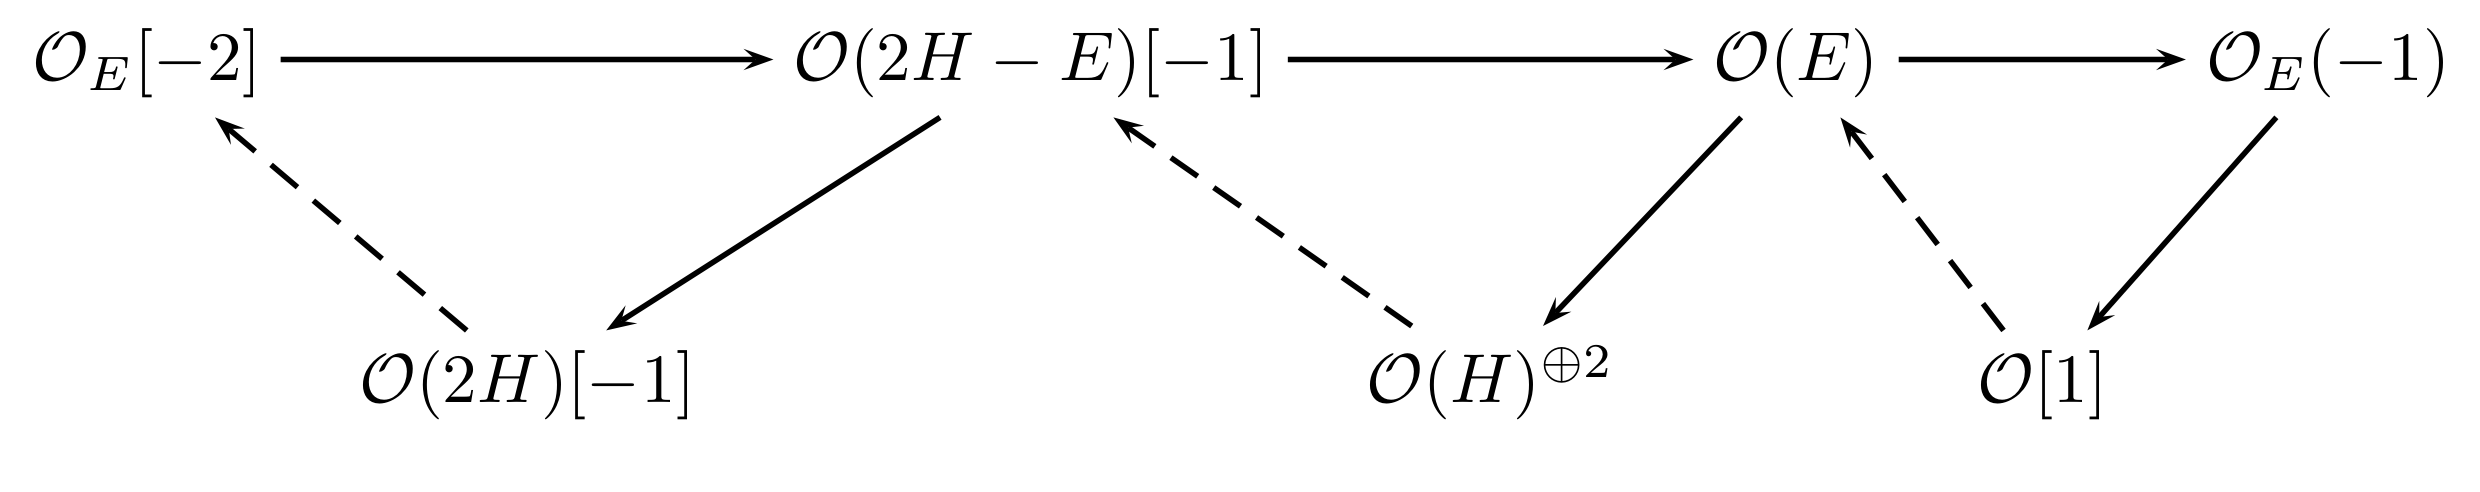
\includegraphics[width=0.82\textwidth]{figures/eq18.20.png}
  \tag{18.20}
\end{equation}

% [Tutor Note: (18.20) 为含虚线斜箭头的图表，preamble 未加载 tikz/tikz-cd，故按页面裁图原样嵌入（work/figures/eq18.20.png）；实线与虚线箭头、上下位置均照原文。]

得到

\begin{equation}
  N \cong \bigl\{\cO_E[-2]\to\cO_E(-1)\to\pi^{*}\cO_p[1]\bigr\} \cong \pi^{*}\cO_p[1] \tag{18.21}
\end{equation}

其中

\begin{equation}
  \cO_p \cong \bigl\{\cO(2H)\to\cO(H)^{\oplus 2}\to\cO\bigr\} \tag{18.22}
\end{equation}

是爆破中心 $p\in\PP^{2}$ 的结构层。

由相干层的导出范畴的半正交分解得到的 Hochschild 上同调正合列

\begin{equation}
  \dots \to \mathrm{HH}^{i}(\cA) \to \mathrm{HH}^{i}(\cA_1)\oplus\mathrm{HH}^{i}(\cA_2) \to \Ext(\phi,\phi) \to \dots \tag{18.23}
\end{equation}

由 [Kuza] 给出。此外，相关结果亦见于 [Han14]。

根据森田理论，Abel 范畴之间的函子 $\phi\colon\mathrm{mod}\,A_1\to\mathrm{mod}\,A_2$ 由 $(A_1,A_2)$ 双模 $M$（左 $A_1$、右 $A_2$）表示为 $X_1\mapsto X_1\otimes_{A_1}M$。在集合

\begin{equation}
  \begin{pmatrix} A_2 & \\ M & A_1 \end{pmatrix}
  := \left\{\,
  \begin{pmatrix} a_2 & 0\\ m & a_1 \end{pmatrix}
  \;\middle|\;
  a_1\in A_1,\ a_2\in A_2,\ m\in M
  \,\right\} \tag{18.24}
\end{equation}

上以

\begin{equation}
  \begin{pmatrix} a_2 & 0\\ m & a_1 \end{pmatrix}
  \cdot
  \begin{pmatrix} a_2' & 0\\ m' & a_1' \end{pmatrix}
  =
  \begin{pmatrix} a_2a_2' & 0\\ m a_2 + a_1 m' & a_1a_1' \end{pmatrix} \tag{18.25}
\end{equation}

定义乘法，所得对象记作 $T(A_1,A_2,M)$，称为三角矩阵代数（triangular matrix algebra）。

\begin{equation}
  \left(
  \begin{pmatrix} u_2 & u_1 \end{pmatrix}
  \begin{pmatrix} a_2 & \\ m & a_1 \end{pmatrix}
  \right)
  \begin{pmatrix} a_2' & \\ m' & a_1' \end{pmatrix}
  =
  \Bigl(
  (u_2a_2)a_2' + (u_1m)a_2' + (u_1a_1)m'
  \quad
  (u_1a_1)a_1'
  \Bigr), \tag{18.26}
\end{equation}

\begin{equation}
  \begin{pmatrix} u_2 & u_1 \end{pmatrix}
  \left(
  \begin{pmatrix} a_2 & \\ m & a_1 \end{pmatrix}
  \begin{pmatrix} a_2' & \\ m' & a_1' \end{pmatrix}
  \right)
  =
  \Bigl(
  u_2(a_2a_2') + u_1(ma_2') + u_1(a_1m')
  \quad
  u_1(a_1a_1')
  \Bigr) \tag{18.27}
\end{equation}

因此，给出 $T(A_1,A_2,M)$-模等价于给出三元组 $(U_1,U_2,\varphi)$：$U_1$ 为 $A_1$-模，$U_2$ 为 $A_2$-模，$\varphi\colon U_1\otimes_{A_1}M\to U_2$ 为 $A_2$-模同态。三元组 $(U_1,U_2,\varphi)$ 与 $(U_1',U_2',\varphi')$ 之间的态射由组 $\psi=(\psi_1,\psi_2)$（其中 $\psi_1\in\Hom_{A_1}(U_1,U_1')$、$\psi_2\in\Hom_{A_2}(U_2,U_2')$）给出，其要求是图表

\begin{equation}
  \begin{array}{c@{\quad}c@{\quad}c}
    U_1\otimes_{A_1}M & \xrightarrow{\ \ \varphi\ \ } & U_2\\[2.6ex]
    \psi_1\otimes\id_M\Big\downarrow & & \Big\downarrow\psi_2\\[2.6ex]
    U_1'\otimes_{A_1}M & \xrightarrow{\ \ \varphi\ \ } & U_2'
  \end{array} \tag{18.28}
\end{equation}

交换。

定义函子 $i_1\colon\mathrm{mod}\,A_1\to\mathrm{mod}\,T(A_1,A_2,M)$ 与 $i_2\colon\mathrm{mod}\,A_2\to\mathrm{mod}\,T(A_1,A_2,M)$ 为

\begin{equation}
  i_1(U_1) = (U_1,0,0),\quad
  i_2(U_2) = (\Hom_{A_2}(M,U_2),U_2),\mathrm{ev}) \tag{18.29}
\end{equation}

则

\begin{align}
  \Hom_{A_2}(\phi(U_1),U_2) &:= \Hom_{A}(i_1(U_1),i_2(U_2)) \tag{18.30}\\
  &\cong \Hom_{A_1}\bigl(U_1,\Hom_{A_2}(M,U_2)\bigr) \tag{18.31}\\
  &\cong \Hom_{A_2}(U_1\otimes_{A_1}M,U_2), \tag{18.32}\\
  \Hom_{A}(i_1(U_1),i_2(U_2)) &= 0 \tag{18.33}
\end{align}

% [Tutor Note: (18.29) 原文的括号作 i_2(U_2)=(\Hom_{A_2}(M,U_2),U_2),\mathrm{ev})，右括号多出一个；按原文照录，疑应为三元组 (\Hom_{A_2}(M,U_2),U_2,\mathrm{ev})。]

在三角矩阵代数中，当 $A_1=\C$ 时，称

\begin{equation}
  A = T(\C,A_2,M) = \begin{pmatrix} A_2 & \\ M & \C \end{pmatrix} \tag{18.34}
\end{equation}

为 $A_2$ 的一点余扩张（one-point coextension）。此外，对于左 $A_2$-模 $N$，称

\begin{equation}
  \begin{pmatrix} A_2 & N\\ & \C \end{pmatrix} \tag{18.35}
\end{equation}

为 $A_2$ 关于 $N$ 的一点扩张（one-point extension）。这些概念由 [Rin84] 引入。

作为构造三角矩阵代数的方法，有对幂等列取有向子代数的做法。若代数 $A$ 的元素列 $(e_1,e_2)$ 满足

\begin{equation}
  e_1^{2} = e_1,\quad e_2^{2} = e_2,\quad e_1e_2 = e_2e_1 = 0,\quad 1 = e_1+e_2, \tag{18.36}
\end{equation}

则称之为 $A$ 的幂等列。对代数 $A$ 的任意幂等元 $e$，$(e,1-e)$ 是幂等列。对幂等列 $(e_1,e_2)$，置

\begin{equation}
  A_1 := e_1Ae_1,\quad A_2 := e_2Ae_2,\quad M := e_1Ae_2,\quad N := e_2Ae_1 \tag{18.37}
\end{equation}

则 $M$ 是 $(A_1,A_2)$ 双模、$N$ 是 $(A_2,A_1)$ 双模，且 $A$ 分解为

\begin{equation}
  A = \begin{pmatrix} A_1 & N\\ M & A_2 \end{pmatrix} \tag{18.38}
\end{equation}

此时置

\begin{equation}
  A^{\to} := T(A_1,A_2,M) \tag{18.39}
\end{equation}

称之为与幂等列 $(e_1,e_2)$ 相伴的 $A$ 的有向子代数（directed subalgebra）。

三角矩阵代数与 Abel 范畴及导出范畴中的 recollement（再粘合）概念密切相关。这是源自 [BBD82] 的概念，关于它可参见例如 [FP04]。

三角矩阵代数的 Hochschild 上同调具有长正合列 [Cib00, GG, MP00, GS02, GMS03]：

\begin{equation}
  \dots \to \mathrm{HH}^{i}(A) \to \mathrm{HH}^{i}(A_1)\oplus\mathrm{HH}^{i}(A_2)
  \to \Ext_{A_1^{\mathrm{op}}\otimes A_2}(M,M) \to \dots \tag{18.40}
\end{equation}

在一点扩张的情形，这些结果更早即已由 [Hap89] 给出。

% CHUNK c08 DONE pages p029–p032
